% Tento soubor nahraďte vlastním souborem s obsahem práce.
%=========================================================================
% Autoři: Michal Bidlo, Bohuslav Křena, Jaroslav Dytrych, Petr Veigend a Adam Herout 2019

% Pro kompilaci po částech (viz projekt.tex), nutno odkomentovat a upravit
%\documentclass[../projekt.tex]{subfiles}
%\begin{document}

\chapter{Úvod}
\label{uvod}
Tato bakalářská práce je věnována návrhu a implementaci digitálního záznamníků s autonomním dokončením záznamu dat při výpadku 
napájení. Požadavek na zařízení vznikl od firmy NXP Semiconductors, konkrétně od týmu zaměřeného na bezdrátové nabíjení, 
ve kterém pracuji. Tento tým působí v České republice, jak v Rožnově pod Radhoštěm tak i v Brně a zároveň má své zastoupení 
v Asii a Severní Americe. NXP Semiconductors je jedním z předních členů WPC (Wireless Power Consortium), organizace zodpovědné 
za definování standardu Qi pro bezdrátové nabíjení. Primární zaměření NXP v této oblasti spočívá ve vývoji referenčních designů 
pro automotive sektor, kde zákazníkům poskytuje řešení určená pro integraci do vozidel.

Zákazníci, kteří využívají referenční designy NXP, pocházejí z celého světa a dostávají téměř hotový produkt, který lze následně 
certifikovat v Qi certifikačních laboratořích. Nicméně i přesto, že jsou referenční designy navrženy podle nejnovějších standardů, 
často dochází k jejich úpravám podle specifických požadavků zákazníků, zejména s ohledem na konkrétní poptávku koncového zákazníka 
(OEM – Original Equipment Manufacturer). Tyto požadavky jsou obvykle shrnuty v RFP (Request for Proposal), kde zákazník specifikuje 
konkrétní požadavky na systém. Tyto úpravy mohou být například realizovány z důvodu snížení ceny nebo zlepšení výkonu, například 
EMC charakteristik a nebo speciální chování bezdrátové nabíječky v krajních situacích. 

Při jakýchkoli úpravách však vznikají nové technické výzvy, a proto NXP poskytuje zákazníkům plnou technickou podporu až do úspěšné 
certifikace. Certifikace probíhá v různých laboratořích po celém světě, avšak ne vždy může být přítomen zaměstnanec NXP, který by 
dohlížel na celý proces a zajistil, že certifikace proběhne hladce. V těchto případech se momentálně tým pro bezdrátové napájení 
spoléhá pouze na záznamy poskytnuté operátorem certifikační laboratoře. Tyto záznamy však pocházejí pouze ze strany přijímače – 
tedy certifikačního zařízení, zpravidla od výrobců Nok9 nebo Granite River Labs (GRL). Ty poskytují některé z důležitých informací, 
bohužel tyto nabídnuté záznamy nezahrnují explicitní informace o chování vysílače. Pokud tedy bezdrátová nabíječka, tedy vysílač 
nějakým testem neprojde, což se občas stává, je často náročné zpětně identifikovat příčinu 
problému. \cite{nxp_wireless_charging_team}

Nezbytným požadavkem na implementaci tohoto záznamníku je i jeho snadná obsluha, neboť zařízení bude poskytováno zákazníkům pro 
účely certifikace. V klasickém scénáři zákazník předá nabíječku i se záznamníkem operátorovi certifikační laboratoře, ten si ji 
připojí k testovanému zařízení. Po skončení testovacího dne operátor záznamník vrátí zákazníkovi, který jej následně připojí k 
počítači a odešle společnosti NXP Semiconductors získané záznamy.


\chapter{Záznam dat}
\label{zaznam_dat}

\section{Počátky záznamu dat}
\label{pocatky}
Lidstvo již od svých počátků mělo potřebu zaznamenávat data, neboť člověk mnohdy dokáže datům přiřadit sémantiku - jejich význam, 
a proměnit je tak v informace. Právě díky nim se lidé mohou učit z minulých zkušeností, předávat znalosti dalším generacím, 
organizovat a podpořit tak neustálý lidský pokrok. 

% Nicméně největším pokrokem ve zaznamenávání dat nastal s příchodem výpočetní techniky.
Po staletí byl záznam dat výhradně manuální. Informace se uchovávaly v rukopisech, knihách či na papírových svitcích, ať už formou 
psaného textu, nebo ručně zapisovaným výsledků pozorování. Přesnost a dostupnost těchto dat byla však omezena kapacitou lidské 
obsluhy a možnostmi mechanických nástrojů.

\begin{figure}[h] % obrazek patent
    \centering
    \includegraphics[width=0.40\textwidth]{obrazky-figures/first_chart_recorder.png}
    \caption{První skutečný grafický záznamník (Chart Recorder) patentovaný Williamem Henrym Bristolem \cite{bristol_chart_recorders}}
    \label{fig:chart_recorder}
\end{figure}

% pripadne to upravit na: Stěžejní změna přišla ve 20. století s rozvojem automatických záznamníků
Stěžejní změna přišla ve 20. století s rozvojem elektrotechniky a nástupem automatických záznamníků, které umožnily primitivní 
sběr dat bez nutnosti lidského zásahu. Namísto ručně zapisovaných měření začaly být hodnoty přenášeny přímo do záznamových 
zařízení, která je dokázala systematicky uchovávat. \cite{origin_of_chart_recorders}

\section{Záznam dat v počátcích elektrotechniky}
\label{zaznam}
Prvními specializovanými záznamníky byly mechanické či elektromechanické zařízení, využívající principu analogového záznamu dat. 
Jejich primárním účelem bylo zaznamenávání fyzikálních veličin, jako je například teplota, tlak, vlhkost nebo vibrace. 
Tyto přístroje využívaly myšlenky mechanického pohyblivého pera, které převádělo naměřenou hodnotu fyzikální veličiny na 
samočinný pohyb. Pro realizaci tohoto pohybu bylo nutné nejprve převést měřenou fyzikální veličinu na mechanický posun. 
Například pro měření teploty se běžně využíval bimetalový pásek, složený ze dvou kovových materiálů s různou hodnotou teplotní 
roztažitelnosti. Při změně teploty docházelo k prohnutí pásku v důsledku rozpínání kovu, čímž bylo rozpohybováno mechanické pero, 
které zapsalo hodnotu na paměťové médium. 

% mechanicky -< samocinny
% pomocí kterého se zapisovala změřená hodnota na paměťové médiu (papírová páska nebo papírový buben)

\begin{figure}[h] % obrazek polygraf
    \centering
    \includegraphics[width=0.50\textwidth]{obrazky-figures/polygraaf.png}
    \caption{Ukázka zařízení patřící do skupiny analogových záznamníků - polygraf \cite{polygraph_picture}}
    \label{fig:polygraaf}
\end{figure}


Tyto přístroje josu běžně používány od druhé poloviny 19. století. Pro již zmíněný záznam teploty lze například využít přístroj 
zvaný cirkulární grafový záznamník (Circular Chart Recorder), dále je hojně využíván polygraf, využívaný jako detektor lži. 
Značnou nevýhodou těchto záznamníků byvá typ paměťového média, na které probíhá zápis hodnot, nejčastěji jim je papírová páska 
nebo papírový buben. Tyto pásky musí být velice často měněny za nové, ještě nepopsané, jelikož výsledné záznamy by se, jinak staly 
značně nepřehledné, pokud by byly popsány vícekrát. \cite{origin_of_chart_recorders}

Největší nevýhodou analogových záznamových systémů je jejich vysoká specializace \footnote{Řešení jsou současně mnohdy 
optimalizovaná pro záznam konkrétního systému.} pro jediný konkrétní typ záznamu. Tyto záznamníky tedy nejsou snadno upravitelné 
pro jiné účely, na rozdíl od digitálních řešení, která umožňují flexibilnější přizpůsobení (například pouhou úpravou programu) k 
sledování monitorované soustavy. Často je v těchto případech nutné využít jiné analogové 
řešení. \cite{analog_signal_and_digital_signal_processing_Tel_System}

Další limitací těchto přístrojů bylo ruční vyhodnocování dat, což bylo mnohdy časově zdlouhavé a také náchylné k chybám. K správné 
interpretaci dat byla často potřeba zkušená obsluha a v některých případech i pomocné měřící pomůcky. Přenos souborů a automatizace 
také nebyla možná, proto jakmile se v polovině 20. století začaly na trh dostávat číslicové systémy, analogové záznamové systémy 
jimi byly postupně nahrazovány. \cite{newcastle_history_of_digital_computers, florian_prechod_a_analog_do_digital}

%Jak obecne probiha princip digitalniho zaznamu dat, co jsou to digitalni data, ze se v dnesni dobe uprednostnuje tento zpusob misto analogoveho zaznamu.

% TODO: Kde napsat co je to vubec zaznamnik? Ze je to pristroj, ktery zpracovava, uklada a pripadne analyzuje data...
\section{Digitální záznam dat}
\label{digitalni_zaznam_dat}
S nástupem číslicových systémů v polovině 20. století došlo k velkému pokroku ve způsobu, jakým jsou data zaznamenávána, 
zpracovávána a uchovávána. Digitální záznam dat postupně nahradil analogové metody, které byly omezené nejen kapacitou paměťových 
médií (viz. kapitola \ref{zaznam}), ale také nutností manuálního vyhodnocení záznamů a obtížným sdílením získaných dat.

\subsection{Princip digitálního záznamu dat}
Digitální záznam dat se oproti analogovému liší způsobem, jakým se v systému obecně pracuje se signály. Zatímco analogový záznam 
pracuje s kontinuálními (spojitými) signály, jak již bylo zmíněno v kapitole \ref{zaznam}, digitální záznam využívá diskrétní 
(číslicové) hodnoty. Tento rozdíl znamená, že analogový signál může nabývat libovolných hodnot v čase, zatímco digitální signál 
je reprezentován jako sada přesně definovaných úrovní, obvykle ve formě binárního kódu (nuly a jedničky).

\begin{figure}[h]
    \centering
    \includegraphics[width=0.95\textwidth]{obrazky-figures/digital_vs_analog.png}
    \caption{Průběh analogového a digitálního signálu}
    \label{fig:digital-vs-analog}
\end{figure}

% TODO: Digitální záznamník může sloužit i pouze pro čistě PC programy? Pokud je zde nejak prijimaci periferie? To by slo primo do CPU

Hlavní výhodou digitálního záznamu oproti analogovému je jeho odolnost vůči šumu a zkreslení. Zatímco analogový signál může být 
postupně degradován například vlivem rušení nebo degradace záznamového média, digitální data lze bezztrátově kopírovat, přenášet 
a rekonstruovat bez snížení kvality.

\subsection{Digitální záznamník}
\label{digitalni_zaznamik}
Digitální záznamník je zařízení nebo softwarový program určený ke sběru, zpracování a ukládání dat ve formě digitálního záznamu. 
Při pohledu na blokové diagramy digitálních záznamníků lze jejich strukturu rozdělit obecně do tří základních komponent, kterými 
jsou přijímající periferie, procesorové jádro a úložiště (viz. obrázek \ref{fig:common-digital-datalogger}). 
\cite{researchgate_general_dataloggger_multiple_sdcards, ieee_digital_sound_recorder_arm_sd_card, ieee_multi_connectivity_datalogger_sd_card}

Prvním klíčovým prvkem digitálního záznamníku je přijímající periferie, která slouží ke sběru vstupních dat. V závislosti na 
konkrétní aplikaci může tato komponenta zahrnovat různé typy vstupních rozhraní, jako jsou sériová rozhraní (UART, SPI, I2C a další) 
síťová rozhraní (Ethernet, Wi-Fi, LoRa, či CAN) nebo analogově-digitální převodníky.\footnote{Vyjímkou jsou specifické monitorovací programy 
mezi, které patří například Windows Task Manager, jež ke svému sběru dat využívají rozhraní pro programování aplikací tzv. kernel API. 
\cite{fourcore_win_process_birth}} \cite{ieee_digital_sound_recorder_arm_sd_card}

\newpage

Druhým hlavním prvkem digitálního záznamníku je procesorové jádro, zajišťující zpracování vstupních dat. Procesorové jádro může být 
jak součástí mikrokontroléru, tak i procesoru, které může mít v tomto případě na starosti jednoduché operace, jako přepočet hodnoty 
z analogově-digitálního převodníku na teplotu podle kalibrační křivky senzoru, přes filtrování šumu a doplňování časových značek 
k naměřeným vzorkům, až po pokročilé analýzy dat - například zpracování signálů pro EKG měření. 
\cite{springer_development_ECG_recorder}

Poslední a také jednou z nejdůležitějších všeobecnou částí digitálního záznamníku je úložiště, kde jsou data uložena pro pozdější 
přenos a zpracování (post-processing). Volba tohoto úložného prostoru závisí na požadavcích aplikace a rozsahu jejího využití - od 
osobních "hobby" projektů až po používání mnoha uživateli. V závislosti na tom lze využít různé technologie od paměťových karet SD 
a eMMC přes interní RAM či flash paměti až po síťová úložiště a cloudové služby. V mnoha případech je také využíván hybridní přístup, 
kdy jsou data nejprve ukládána do interní paměti záznamníku (například RAM úložiště) a následně dávkově přenášena na trvalé médium 
(viz. kapitola \ref{fig:batch-processing}) nebo odesílána přes síť. \cite{rta_local_vs_cloud}
    

\begin{figure}[h]
    \centering
    \includegraphics[width=0.95\textwidth]{obrazky-figures/common_digital_datalogger_scheme.png}
    \caption{Obecné schéma digitálního záznamníku}
    \label{fig:common-digital-datalogger}
\end{figure}

Digitální záznamník poskytuje výstupy, kterými jsou organizovaná data, jež mohou být dále analyzována, vizualizována nebo 
zpracovávána jinými systémy. Jakou podobu mají výstupní data, tedy jejich formát, opět závisí na konkrétních požadavcích aplikace. 
Jedním je volba podle typu typ uložiště, jedná-li se o lokální úložný prostor, například paměťovou kartu, využívají se obecně 
soubory různých formátů, jako třeba textové nebo binární formy. Zatímco cloudová řešení využívají objektové formáty nebo lehké 
databázové systémy. Dále záleží, jakým způsobem bude proveden přenos dat, pokud bude využita síťová komunikace třeba pomocí MQTT 
či HTTP, je vhodné data uspořádávat do serializované podoby, zatímco při zvolení přenosu po sériové lince je naopak vhodnější a 
efektivnější využít opět některý z binárních formátů. Důležitou roli hrají i požadavky na následné zpracování (post-processing) a 
interpretaci dat v jiných systémech či aplikacích k tomu určeným. Například pro nazírání na data z pohledu časových řad může být 
vhodné využít formáty, které jsou kompatibilní s například databázovým systémem TimescaleDB. V dalších případech může být efektivní 
využít knihovny pro zpracování a analýzu dat, například Pandas v prostředí Pythonu, které umožňují rychlou manipulaci s velkým 
objemem strukturovaných dat, v takových případech je tedy zase lepší strukturovat data podle formátu CSV. 
\cite{medium_optimalization_iot_data_storage_timescaledb}

\newpage

\begin{figure}[h]
    \centering
    \includegraphics[width=0.95\textwidth]{obrazky-figures/advanced_architecture_of_datalogging_3.png}
    
    \caption{Schéma pokročilého digitálního záznamníkíku s cloudovým uložištěm postavený na streamingové platformě Kafka \cite{confluent_advanced_datalogging, influxdata_advanced_datalogging_mmqt}}
    \label{fig:advanced-architecture-of-datalogging}
\end{figure}


Způsobů, jak lze digitální záznamník sestavit, existuje mnoho, přičemž volba konkrétní architektury závisí na požadavcích dané 
aplikace. Velice často se však skládá z výše představených komponent. 

\subsection{Digitální záznam v počítačovém systému}
Digitální záznamníky lze implementovat na počítačových systémech, které představují softwarová řešení, sloužící ke sběru, 
zpracování a případnou archivaci dat. Tyto systémy obvykle také vycházejí ze struktury obecného číslicového záznamníku popsaného 
v kapitole \ref{digitalni_zaznamik}. Vstupní data přicházejí často z periferií jako je například síťová karta či senzorických 
zařízení, ale mohou také pocházet ze speciálních "pseudo" zařízeních obsahující stavy aplikací běžících na daném počítači. 
Procesor, který tato data příjímá tak je obvykle nejen zpracovává, ale často i nějakým způsobem vyhodnocuje, jelikož disponuje 
dostatečným výpočetním výkonem pro pokročilé operace. Výsledkem těchto operací procesoru nad daty mohou být informace o aktuálním 
stavu sledovaného systému, které mohou být využity pro monitorování a další rozhodovací procesy. 
\cite{linux_in_action_log_and_monitoring}

\subsection{Digitální záznam na platformě mikrořadiče}
Pro návrh a implementaci 

\section{Koncepty využívané ke zpracování dat digitálních záznamníků} 
Digitální záznamníky často bývají implementovány na platformě MCU, která dokáže poskytnout dobrý kompromis mezi cenou a výkonem, 
nicméně je nezbytné zohlednit specifická omezení a vlastnosti daného mikrokontroléru. Oproti počítačovým systémům mají MCU omezené 
výpočetní a paměťové zdroje, což vyžaduje důkladný návrh architektury systému. Proto je i nutné volit takové metody, které mohou 
minimalizovat latenci, spotřebu energie a nároky na paměť, a zároveň zajistí spolehlivý provoz v reálném čase.

\subsection{Vícenásobná vyrovnávací paměť (multiple-buffering)}
Jedním z častých konceptů využívaných v implementaci digitálních záznamníků je použití vícenásobné vyrovnávací paměti. Tento 
koncept je převážně známý díky algoritmům využívaným v oboru počítačové grafiky. Grafický čip musí zpracovat velké množství dat 
za krátký časový úsek, proto algoritmus zpracování dat využívá dvě vyrovnávací paměti - přední vyrovnávací paměť, takzvaný 
front-buffer, jež je využívána pro zobrazení aktuálního snímku a zadní vyrovnávací paměť, ve které čip připravuje nový obsah. 
Výsledný obsah tak může být plynule vykreslen bez artefaktů a trhání. Jakmile je nový snímek kompletní, vyrovnávací paměti se 
prohodí. \cite{double_buffering_model}

Obdobný mechanismus se využívá i v digitálních záznamnících, kde slouží k zajištění kontinuálního sběru dat bez výpadků. Zatímco 
jeden buffer přijímá nová data ze vstupní periferie (například analogově-digitálního převodníku či jiných vstupů), druhý buffer 
je současně zpracováván nebo ukládán na úložné médium. Tím se minimalizuje riziko ztráty dat způsobené časovou prodlevou při 
jejich zpracování nebo zápisu.

\begin{figure}[h]
    \centering
    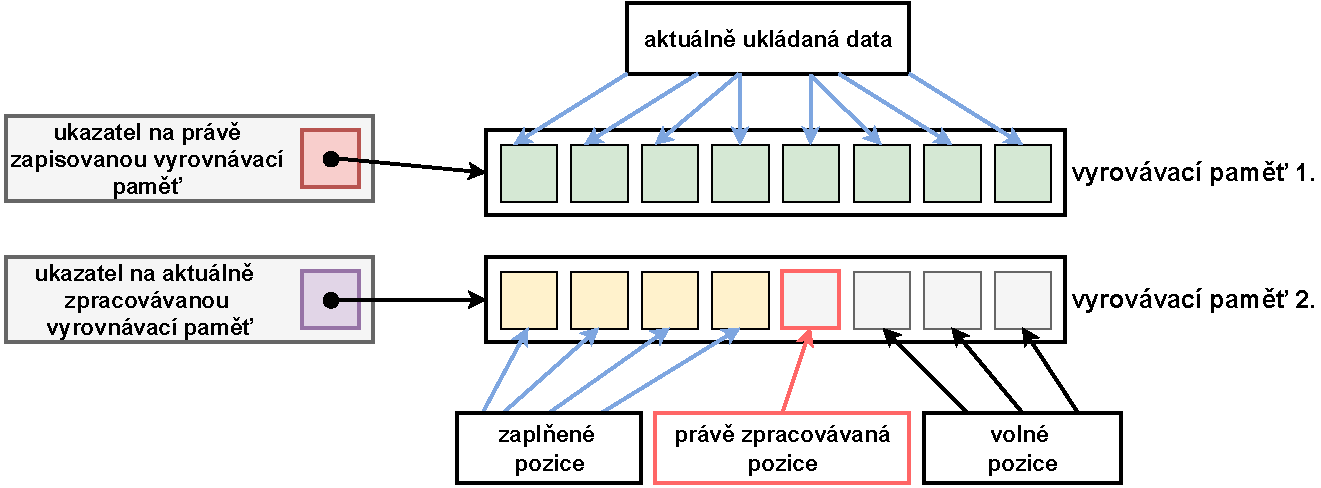
\includegraphics[width=0.95\textwidth]{obrazky-figures/multiple_buffering-1-1.png}
    
    \caption{Schéma principu práce s vícenásobnou vyrovnávací paměťí - náhodný stav}
    \label{fig:multiple-buffering-1}
\end{figure}

Důležitou vlastností tohoto algoritmu je jeho nízká operační režijní náročnost. Plynulý chod zpracování dat je zajištěn bez 
nutnosti fyzického přenosu obsahu mezi vyrovnávacími pamětmi. Místo toho se využívají ukazatele (pointery), které směřují na 
počáteční adresy jednotlivých bufferů. Jakmile je sběrný buffer (Back Buffer) naplněn, ukazatele se prohodí~–~back buffer se 
stane zpracovávaným bufferem (Front Buffer) a původní front buffer se uvolní pro další sběr dat.

\begin{figure}[h]
    \centering
    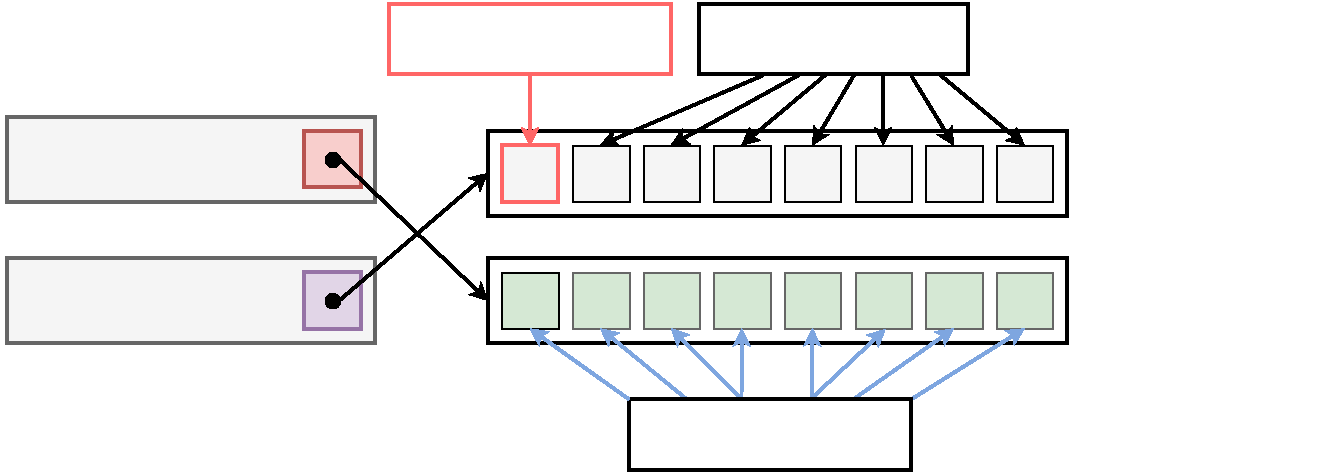
\includegraphics[width=0.90\textwidth]{obrazky-figures/multiple_buffering-2-2.png}
    
    \caption{Schéma principu práce s vícenásobnou vyrovnávací paměťí - přeřazení ukazatelů}
    \label{fig:multiple-buffering-2}
\end{figure}

Tato metoda nachází významné uplatnění zejména v systémech pracujících v reálném čase, kde dochází k příjmu velkého objemu dat 
v krátkých časových intervalech a kde doba zpracování nesmí překročit dobu sběru dat. Využitím vícenásobné vyrovnávací paměti se 
minimalizuje latence zpracování a současně se snižuje riziko přetečení paměťového prostoru. \cite{buffering_chang}

Nicméně, žádný algoritmus není dokonalý a i tato metoda má své nevýhody, které je třeba zmínit. Vyrovnávací paměti jsou zpravidla 
implementovány softwarově, nikoliv hardwarově, což vede k zvýšeným nárokům na paměťové prostředky, obzvlášť v segmentu volatilní 
paměti (SRAM/DRAM) kde jsou buffery uložené. \cite{basics_of_digital_forensics}
% TODO: Je tedy vhodne si promyslet zda zdroje MCU budou dostacovat.

\subsection{Dávkové zpracování (batch processing)}
Další princip, jež je využívaný v implementacích digitálních záznamníků, souvisí s typem uložišť, na které jsou získaná data 
zaznamenávána. Některé typy nevolatilních pamětí, například NAND Flash paměť, jež umožňují uchování dat i po odpojení napájení. 
Tyto druhy paměti jsou organizovány do bloků (viz. obrázek \ref{fig:batch-processing}), přičemž bloky jsou následně rozděleny na 
menší jednotky zvané sektory. Velikost sektoru obvykle bývá 512 bajtů či 4096 bajtů, v závislosti na typu média a jeho architektuře. Tato bloková struktura umožňuje účinnou správu prostoru, které uložiště nabízí, ale současně vyžaduje specifický způsob zápisu/čtení dat, které je pouze umožněno na úrovni celých bloků.  \cite{tech_target_nand_flash, non_volatile_memories}

Dávkové zpracovátí tohoto chování paměti využívá, data se tedy nejprve shromažďují ve volatilní paměti - například RAM a teprve po 
naplnění určitého objemu (celého bloku či jeho násobku) dojde k jejich zápisu na konečné paměťové médium.

\begin{figure}[h]
    \centering
    \includegraphics[width=0.70\textwidth]{obrazky-figures/batch_processing.png}
    
    \caption{Organizace bloku nevolatilní paměti \cite{ieee_relationships_among_region_segment_frame_and_cluster}}
    \label{fig:batch-processing}
\end{figure}


\subsection{Cirkulární buffer}
Cirkulární buffer (circular buffer), někdy také označovaný jako kruhový nebo cylindrický buffer, je datová struktura, která 
funguje na principu FIFO fronty (First-In, First-Out) a považuje tuto paměť za kruhovou. Tento přístup je často využíván k řešení 
problému jednoho producenta a konzumenta (producent-consumer problem), kde jedno vlákno je konzument a druhé producent. Například 
ve vestavěných zařízeních, jednímž vláken je rutina obsluhy přerušení, která čte data ze senzoru a druhým vláknem je hlavní smyčka 
události.  \cite{embedjournal_ring_buffer}


\begin{figure}[h]
    \centering
    \includegraphics[width=0.90\textwidth]{obrazky-figures/circular_buffer_titles.png}
    
    \caption{Cirkulární vyrovnávací paměť}
    \label{fig:circular-buffer}
\end{figure}

Princip činnosti cirkulárního bufferu spočívá v použití dvou ukazatelů - zápisový ukazatel (head) a čtecí ukazatel (tail). Ukazatel 
head vždy směřuje na pozici, kam bude zapisován následující prvek, zatímco ukazatel tail ukazuje na pozici, ze které bude čtena 
následující hodnota. Pokud ukazatel head dosáhne konce pole, vrací se na jeho začátek, čímž je zajištěna kruhová povaha struktury. 
Při plném bufferu lze zvolit dvě strategie – přepsání nejstarších dat nebo odmítnutí nových vstupů, přičemž výběr závisí na konkrétní aplikaci. \cite{embedjournal_ring_buffer, medium_ring_buffer}

Z hlediska časové složitosti nabízí cirkulární buffer konstantní časovou složitost - O(1) pro základní operace, jako je zápis 
(enqueue) a  čtení (dequeue). Tato efektivita je dána tím, že se při zápisu a čtení dat není potřeba přesouvat prvky v paměti, 
ale stačí pouze inkrementovat ukazatele s využitím operace modulo. Pokud jde o prostorovou složitost, velikost cirkulárního bufferu 
je určena předem – zpravidla jde o staticky alokované pole o velikosti n prvků, což odpovídá složitosti O(n), kde n je maximální 
počet prvků, které může buffer pojmout. \cite{petrungaro_ring_buffer_complexity}

\subsection{Nízko-energetické režimy (low-power modes)}
Energetická efektivita je jedním z klíčových parametrů obecně vestavěných zařízení, tedy i digitálních záznamníků implementovaných 
na platformě MCU, zejména pokud jsou napájeny z baterií či jiných omezených zdrojů energie (například energy harvesting). 
Minimalizace spotřeby bývá v těchto případech realizována využitím nízkoenergetických režimů (low-power modes), které umožňují 
zařízení přejít do stavu s minimální energetickou náročností během nečinných period. V praxi mnoho digitálních záznamníků nemusí 
provádět měření a záznam dat nepřetržitě. Například záznamník teploty může v pravidelných intervalech provést měření, uložit 
naměřenou hodnotu, přejít do režimu nízké spotřeby a po uplynutí definovaného časového intervalu nebo při vyskytnutí speciální 
události přejít do aktivního režimu. \cite{analog_devices_low_power_modes}

Průběh takového cyklického chování spotřeby mikrokontroléru, kde se střídají fáze měření a spánku s pravidelnou periodou měření 
teploty, je znázorněn na obrázku \ref{fig:low-power-modes} níže.

\begin{figure}[h]
    \centering
    \includegraphics[width=0.90\textwidth]{obrazky-figures/low_power_modes.png}
    
    \caption{Graf znázorňujíci dynamiku spotřeby mikrokontroléru v průběhu času při využití aktivního a nízkoenergetického režimu}
    \label{fig:low-power-modes}
\end{figure}

Ačkoliv nízkoenergetické režimy přinášejí značné úspory energie a jsou nezbytné pro zařízení napájená z baterií, u dataloggerů s 
velkým objemem zaznamenávaných dat mohou představovat významná omezení. Tyto režimy sice snižují energetickou náročnost systému, 
avšak zároveň omezují schopnost mikrokontroléru rychle reagovat na události. Spánkové stavy, které minimalizují spotřebu energie, 
často vedou k delšímu zpoždění při probuzení a nižší dostupnosti kritických periferií. V aplikacích, kde je vyžadována okamžitá 
odezva na externí podněty nebo nepřetržité zpracování velkého množství dat, může tento faktor negativně ovlivnit spolehlivost a 
efektivitu záznamníku. \cite{embedded_low_power_modes}

V těchto případech je proto nutné zvážit provozní podmínky a očekávanou dostupnost systému. Pokud záznamník pracuje s velkým 
datovým tokem a má možnost být připojen po dobu záznamu stále k externímu napájení, může být výhodnější upustit od implementace 
nízkoenergetických režimů a místo toho optimalizovat architekturu systému pro nepřetržitý provoz s důrazem na výkon a rychlou 
odezvu. \cite{analog_devices_low_power_modes}

\section{Typy médií pro záznam dat}
Hard disk, vyhody nevyhody,...

\chapter{Návrh digitálního záznamníku}


\section{Existujících řešení digitálních záznamníku}


\section{Výběr vhodné platformy}
Neni vhodne implementovat zaznamnik na pocitacovem systemu, je treba zvolit stragii implementace na mikroradici, porovnat FRDM-MCXN947, Arduino, Raspberry

\subsection{FRDM-MCXN947}

\subsection{Arduino}

\subsection{Linux based - Raspberry}

Pripraven i popis jadra ARM Cortex-M33, ktere vyuziva FRDM-MCXN947.

% ----------------------------------------------------
% DALSI NAZVY: Volba datového úložiště, Výběr externího uložiště pro záznam dat, Možnosti způsobu ukládání získaných dat
\section{Přístupy k ovládaní úložiště}
Obecný popis, proč je potřeba externí uložiště, že by se data mohla ukládat i v RAM paměti, ale že by tam moc dlouho nevydržela, 

\subsection{SDHC}

\subsection{SPI}

\subsection{Quad-SPI flash}


% ----------------------------------------------------
% DALSI NAZVY: Volba datového úložiště, Výběr externího uložiště pro záznam dat
\section{Možnosti správy dat - souborové systémy} 
Obecný popis, souborový systém je zodpovědný za organizaci, správu a přístup k datům na zvoleném úložném médiu.

\subsection{FATFS}

\subsection{Chan FATFD}

\subsection{LittleFS}


% ----------------------------------------------------

\section{Výběr řízení přístupu k získaným datům}

\subsection{USB Mass Storage}

\subsection{Media Transfer Protocol}

\subsection{Human Interface Device}

% ----------------------------------------------------
\section{Výběr zdroje času}

\subsection{Obvod reálného času}

\subsection{Interní časovač}

\subsection{Bezdrátová komunikace (GPS/NTP)}

% ----------------------------------------------------
\section{Výber přístupu řízení běhu aplikace}
Srovnani obecne bare-metal a RTOS.


\subsection{Bare-Metal}

% TODO: Zde to asi spis rozdelit na Baremetall vs. RTOS a pak uvest priklady jako FreeRTOS a ZephyrRTOS
\subsection{RTOS}
\subsubsection{FreeRTOS}
Konkretní výhody a nevýhody FreeRTOS

\subsubsection{ZephyrRTOS}
Konkretní výhody a nevýhody ZephyrRTOS

% ----------------------------------------------------

\section{Architektura systému digitálního záznamníku}
Popis architektury na základě vybraných komponent. Popis blokového diagramu.

\begin{figure}[h]
    \centering
    \includegraphics[width=0.90\textwidth]{obrazky-figures/architecture-block-diagram.png}
    
    \caption{Výsledná architektura digitálního záznamníku}
    \label{fig:low-power-modes}
\end{figure}

% ----------------------------------------------------

\section{Volitelné rozšíření}
\subsection{Měření teploty}

% ----------------------------------------------------

\subsection{Řešení problému synchronizace času}

% ----------------------------------------------------

\chapter{Realizace hardwaru}
Popis co všechno je již na platformě FRDM MCXN947, z toho ti vyplyne co všechno bude ještě muset nabízet expanzní deska.
\section{Základová deska}
\section{Expanzní deska}

\section{Mechanická část}
Jak jsem měřil spotřebu, jak jsem spočítal hodnoty kondenzátorů

\chapter{Softwárová implementace}

\section{Záznamové vlákno}

\section{USB Mass Storage vlákno}

\section{Signalizace stavu systému}

% ==================================================== 
\chapter{Testování systému}
Obecne proc je potreba testovat, jake jsou moznost testovani a validace vestavenych systemu

% ----------------------------------------------------

\section{Testování a validace}

\subsection{Funkcionální testování}
Popis skriptů pro automatické testování, popis výsledků, atd, ...

\subsection{Kontrola bezpečnosti kódu}
MISRA

% ----------------------------------------------------

\section{Limitace systému}
\label{limitace}

% ----------------------------------------------------

\section{Možná rozšíření záznamníku}
\label{mozne_rozsireni}

\chapter{Závěr}
\label{zaverPrace}


%===============================================================================

% Pro kompilaci po částech (viz projekt.tex) nutno odkomentovat
%\end{document}
